  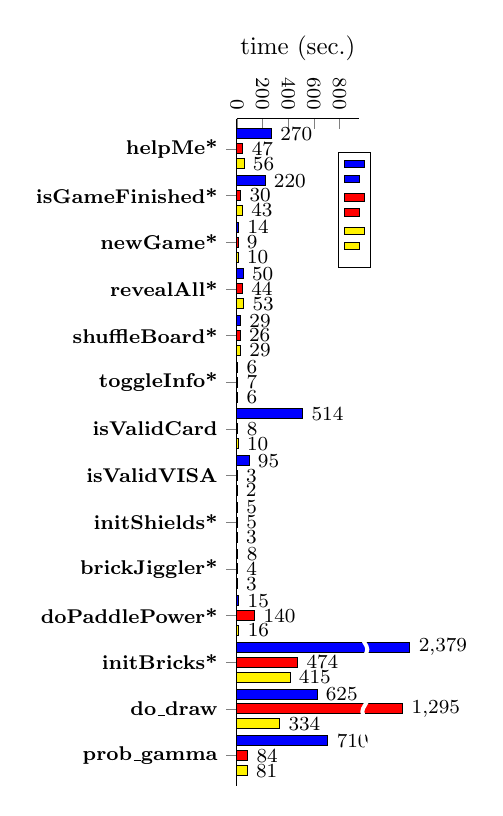
\begin{tikzpicture}[scale=0.9,rotate=-90]

    \begin{axis}[
        every axis plot post/.style={/pgf/number format/fixed},
        ybar,
        ymin=0,ymax=950,
        width=11cm,height=3.3cm,
        bar width=4pt,
        enlarge x limits=0.05,
        legend style={rotate=45,anchor=north west,font=\footnotesize,legend columns=-1,at={(0.05,1.1)}},
        legend cell align={left},
        ylabel={time (sec.)},
        symbolic x coords={helpMe*,isGameFinished*,newGame*,revealAll*,shuffleBoard*,toggleInfo*,isValidCard,isValidVISA,initShields*,brickJiggler*,doPaddlePower*,initBricks*,do\_draw,prob\_gamma},
        xtick=data,
        restrict y to domain*=0:1350, % Cut values off at 14
        visualization depends on=rawy\as\rawy, % Save the unclipped values
        after end axis/.code={ % Draw line indicating break
          \draw [ultra thick, white, decoration={snake, amplitude=1pt}, decorate] (rel axis cs:0,1.05) -- (rel axis cs:1,1.05);
        },
        nodes near coords={%
          \pgfmathprintnumber{\rawy}% Print unclipped values
        },
        every node near coord/.append style={rotate=90,anchor=west,font=\footnotesize},
        % every node near coord/.append style={font=\footnotesize},
        axis lines*=left,
        clip=false,
        x tick label style={rotate=90,anchor=east,font=\footnotesize\bfseries},
        y tick label style={font=\footnotesize}
      ]
      \addplot[fill=blue] coordinates {(helpMe*,270) (isGameFinished*,220) (newGame*,14) (revealAll*,50) (shuffleBoard*,29) (toggleInfo*,6) (isValidCard,514) (isValidVISA,95) (initShields*,5) (brickJiggler*,8) (doPaddlePower*,15)  (initBricks*,2379) (do\_draw,625) (prob\_gamma,710)};
      \addplot[fill=red] coordinates {(helpMe*,47)  (isGameFinished*,30)  (newGame*,9)  (revealAll*,44) (shuffleBoard*,26) (toggleInfo*,7) (isValidCard,8)   (isValidVISA,3)  (initShields*,5) (brickJiggler*,4) (doPaddlePower*,140) (initBricks*,474) (do\_draw,1295) (prob\_gamma,84)};
      \addplot[fill=yellow] coordinates {(helpMe*,56)  (isGameFinished*,43)  (newGame*,10) (revealAll*,53) (shuffleBoard*,29) (toggleInfo*,6) (isValidCard,10)  (isValidVISA,2)  (initShields*,3) (brickJiggler*,3) (doPaddlePower*,16) (initBricks*,415) (do\_draw,334) (prob\_gamma,81)};
      \legend{$\Random$,$\Genetic$,$\RGenetic$}
    \end{axis}
  \end{tikzpicture}
